\chapter{Greenhouse Model}
\label{cha:greenhousemodel}

A greenhouse is a building designed to permit growth of plants and crops in regions and seasons, in which they could not naturally survive. By controlling the climatic, biotic, nutrition and cultural management optimal agricultural conditions can be obtained. The goal is the optimization of the profit by producing the maximum amount of a product with the highest quality at minimal cost.

First, a overview of the model is given (\cref{sec:model_overview}).
Afterwards, the model equations for inside air temperature (\cref{sec:temp}) and inside air humidity (\cref{sec:hum}) are presented.
%\cref{sec:application} explains how the model is implemented in different model predictive control (MPC) approaches.

\section{Model overview}
\label{sec:model_overview}

The several elements composing a greenhouse are linked by energy, mass and information flows.
This results in a high level of complexity which makes the division into subsystems and their examination necessary.
\cref{fig:greenhouse_subsystems} illustrates a possible division into subsystems and how they affect each other.
For example a moist and hot weather may increase the growth of vermin which might feed on the leaves of the crop.

\begin{figure}[t]
\begin{center}
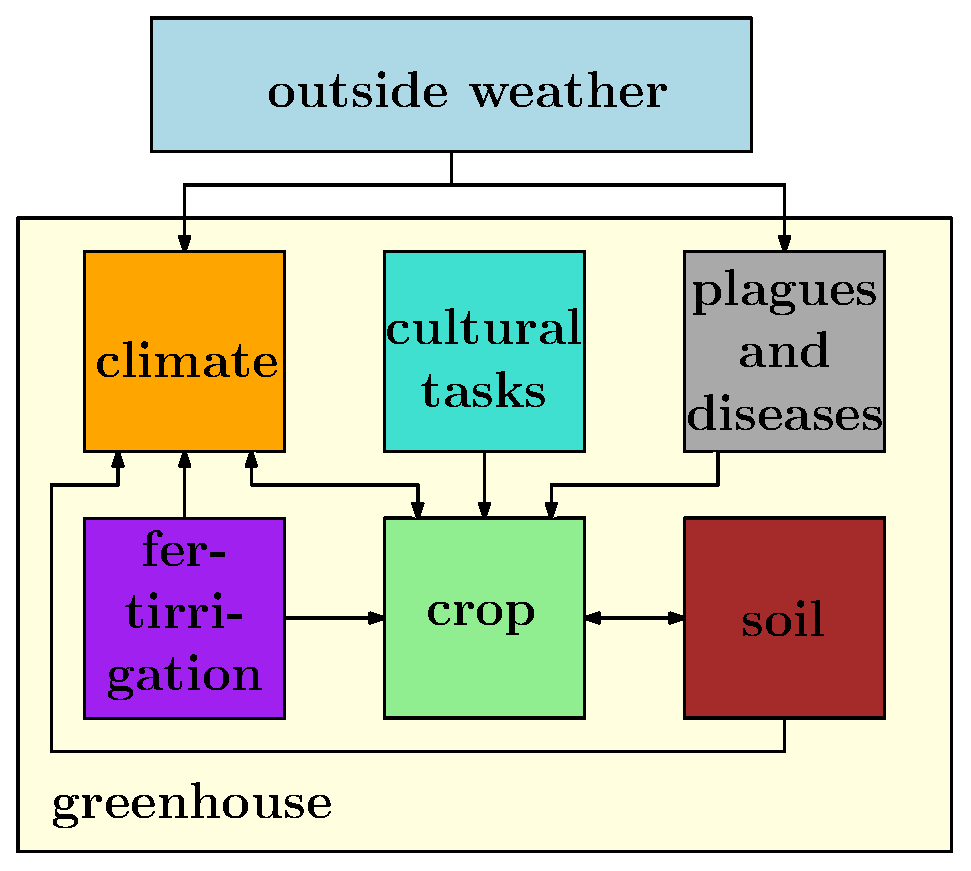
\includegraphics[width=.7\textwidth]{../Figures/subsystems.eps}
\caption{Concept of a greenhouse and its subsystems}
\label{fig:greenhouse_subsystems}
\end{center}
\end{figure}

Generally, three kinds of variables can be distinguished as \cref{fig:greenhouse} shows: Inputs are variables that can be controlled directly (e.g. heating), disturbances are variables affecting the crop growth and the inside air conditions but cannot be manipulated (e.g. outside weather) and outputs are the controlled variables (e.g. inside air temperature).
The automated control of a greenhouse requires the necessary set of sensors and actuators.

\begin{figure}[t]
\begin{center}
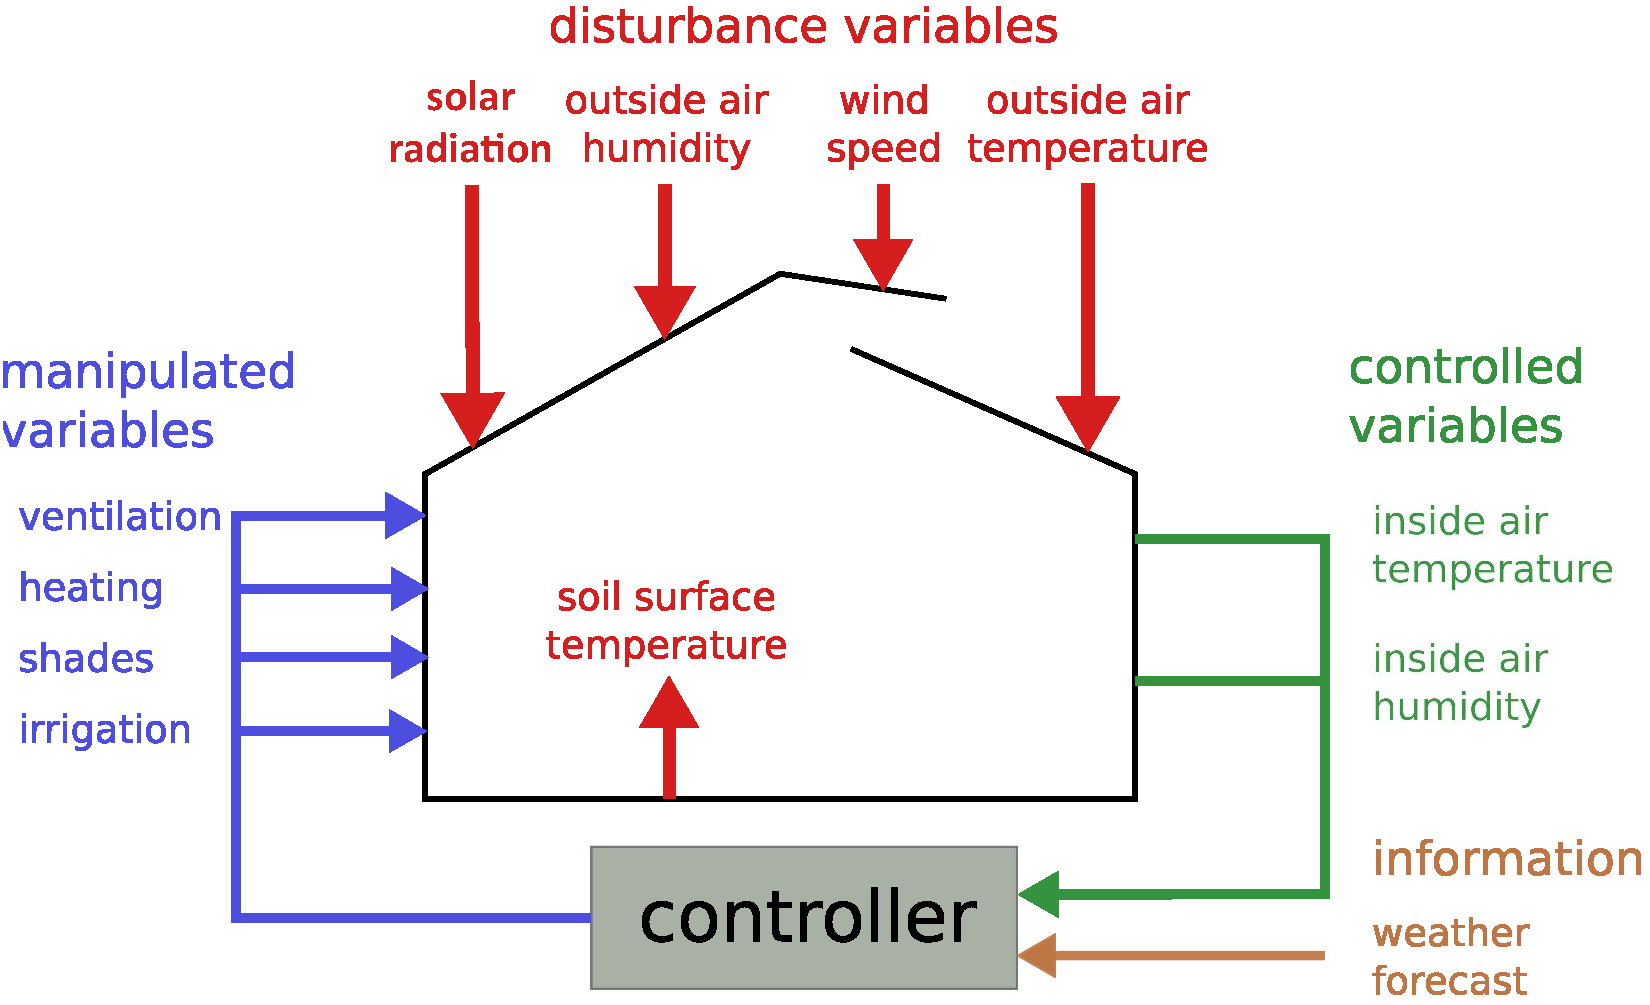
\includegraphics[width=\textwidth]{../Figures/greenhouse_quer.pdf}
\caption{Greenhouse climate control scheme}
\label{fig:greenhouse}
\end{center}
\end{figure}

The greenhouse model used is a nonlinear pseudo-physical climate model from chapter 2.1.2 of \cite{Rodriguez.2015}.
This means it is a simplified model derived from high-complex ones that has some physical sense.
To model the greenhouse, nine exogenous and two endogenous variables are considered.
The system states are inside air temperature $X_{T_{a,a}}$ and inside air humidity $X_{H_{a,a}}$.
The exogenous variables can be divided into disturbance variables and control inputs.
The disturbance variables are outside air temperature $D_{T,e}$, relative outside air humidity $D_{H,e}$, wind speed $D_{ws,e}$, global radiation $D_{rs,e}$ and the soil surface temperature $D_{T,ss}$.
The manipulated variables are the vents opening position $U_{ven}$, the shade screen position $U_{shd}$, the heat from the air heating system $U_{heat}$ and the water from the moisturisation system $U_{hum}$.

The following assumptions and simplifications were done:
\begin{itemize}
	\item An ordinary differential equation (ODE) model is used instead of a partial differential equation (PDE) one, because perfect air mixing behaviour is assumed
	\item Heat transfer coefficients are considered constant in time and temperature
	\item The physical properties of air, such as density or specific heat, are considered constant
	\item For heating no specific system like heat pipes or air heater is assumed, therefore it is only a quantitative measure for the energy usage
	\item For moisturisation no specific system like fogging or misting is assumed, therefore it is only a quantitative measure for the water consumption
\end{itemize}

The two states are each described by nonlinear ODEs in which the ventilation flux $V_{ven,flux}$ has a crucial impact.
The ventilation flux is given by:
\begin{equation}\label{eq:venflux}
V_{ven,flux} = D_{ws} \cdot \alpha \cdot U_{ven}^\beta + c_{loss} \cdot D_{ws} + c_{leak},
\end{equation} 
where $\alpha$ and $\beta$ are empirical parameters, $c_{loss}$ is the influence factor of the windspeed when the vents are closed and $c_{leak}$ is the leakage of warmth due to imperfect sealing.
In the following two sections the two ODEs are explained.
The value of the parameters are gathered in \cref{sec:physical_params}.
%%%%%%%%%%%%%%%%%%%%%%%%%%%%%%%%%%%%%%%%%%%%%%%%%%%%%%%%%%%%%%%%%%%%%%%%%%%%%
\section{Internal air temperature model}
\label{sec:temp}
The greenhouse air temperature is modelled by the following balance:
\begin{equation}\label{eq:temp}
\begin{split}
\frac{dX_{T,a}}{dt} &= \frac{c_{area,ss} \cdot c_{sph,a} \cdot c_{den,a}}{c_{vol,g}} \cdot \left(Q_{sol,a} + Q_{cnv,ss-a} + Q_{heat-a} \right.\\
		& \left. + Q_{cnv-cnd,a-e} - Q_{ven,a-e} - Q_{loss,a-e} - Q_{trp,cr}\right),
\end{split}
\end{equation}
where $c_{area,ss}$ is the surface area of the soil, $c_{sph,a}$ is the specific heat and $c_{den,a}$ is the density of the air.
The heat fluxes $Q_{(\cdot)}$ are described in the following paragraphs.

The solar radiation absorbed by the air $Q_{sol,a}$ is given by:
\begin{equation}\label{eq:rs}
Q_{sol,a} = c_{asw,a} \cdot V_{tsw,g} \cdot D_{rs,e} \cdot \left( 1 - U_{shd} \right),
\end{equation}
where $c_{asw,a}$ is the short-wave absorption coefficient of the greenhouse air. $V_{tsw,g}$ is the short wave heat transmission coefficient depending on the cover, its whitening state and the shading screen.

The heat transfer between the soil surface and the inside air is depending on the temperature difference between soil surface temperature $D_{T,ss}$ and inside air temperature $X_{T,a}$:
\begin{equation}\label{eq:ss}
Q_{cnv,ss-a} = c_{cnv,ss-a} \cdot (D_{T,ss}-X_{T,a}),
\end{equation}
where $c_{cnv,ss-a}$ is the constant convection coefficient.

This process is proportional to the temperature difference between outside air temperature $D_{T,e}$ and inside air temperature $X_{T,a}$:
\begin{equation}\label{eq:a-e}
Q_{cnd-cnv,a-e} = c_{cnd-cnv,a-e} \cdot (D_{T,ss}-X_{T,a}),
\end{equation}
where $c_{cnd-cnv,ss-a}$ is the thermal loss coefficient for convection and conduction processes.

The Heat transfer to the outside air due to ventilation and infiltration are described by:
\begin{equation}\label{eq:loss}
\begin{split}
Q_{ven,a-e} + Q_{loss,a-e}& = \\
\frac{c_{den,a} \cdot c_{sph,a}}{c_{area,ss}} \cdot &V_{ven,flux} \cdot (X_{T,a}-D_{T,e}).
\end{split}
\end{equation}
%%%%%%%%%%%%%%%%%%%%%%%%%%%%%%%%%%%%%%%%%%%%%%%%%%%%%%%%%%%%%%%%%%%%%%%%%%%%%%%%%%%%%%%%%%%%%%%%%%%%%%%%%%%%%%%%%%%%%%%%%%%%%%%%%%%%%%%%%%%%%%%%%%%%%%%%%%
%%%%%%%%%%%%%%%%%%%%%%%%%%%%%%%%%%%%%%%%%%%%%%%%%%%%%%%%%%%%%%%%%%%%%%%%%%%%%%%%%%%%%%%%%%%%%%%%%%%%%%%%%%%%%%%%%%%%%%%%%%%%%%%%%%%%%%%%%%%%%%%%%%%%%%%%%%

\section{Internal air humidity model}
\label{sec:hum}
The internal air humidity is modelled by the following balance:
\begin{equation}\label{eq:hum}
\frac{dX_{H_{a,a}}}{dt} = \frac{c_{area,ss}}{c_{den,a} \cdot c_{vol,g}} \cdot \left(M_{trp,cr}-M_{ven,a-e}+U_{hum}\right),
\end{equation}
where the two sources of water vapor are the crop transpiration $M_{trp,cr}$ and the injections of the moisturisation system $U_{hum}$, while the loss of water vapor is due to exchange of air with the outside through ventilation.

For the water vapour increase due to the crop tomato a balance $M_{trp,cr}$ based on the Penman-Monteith equation is used:
\begin{equation}\label{eq:crtp}
\begin{split}
M_{trp,cr} &= \frac{1}{V_{r,trp}}\Big(V_{hsat,a} \\
           &+ \frac{1}{c_{den,a}}\frac{V_{ssvp}}{c_{psyco}}\frac{V_{r,bl}}{2D_{LAI}}\frac{V_{rn,cr}}{V_{lt,vap}}-X_{Ha,a} \Big),
\end{split}
\end{equation}
where $c_{psyco}$ is the thermodynamic psychometric constant, $D_{LAI}$ is the leaf area index of the tomato crop and $c_{den,a}$ is the densitiy of the inside air.

The thermodynamic psychometric constant $c_{psyco}$ is calculated by:
\begin{equation}\label{eq:psyco}
c_{psyco} = \frac{c_p \cdot p}{\lambda_v \cdot MW_{ratio}},
\end{equation}
where $p$ is the atmospheric pressure, $\lambda_v$ is the latent heat of water vaporization, $c_p$ is the specific heat of air at constant pressure and $MW_{ratio}$ is the ratio of molecular weight of water vapour and dry air.

The water concentration of the air at saturation $V_{hsat,a}$ is calculated with Teten's formula:
\begin{equation}\label{eq:vhsat}
V_{hsat,a} = 611.2 \cdot exp\left({\frac{\frac{17.62 \cdot X_{T_{a,a}}}{243.12 + D_{T,e}}}{R_D \left(273.2 + X_{T_{a,a}}\right)}}\right),
\end{equation} where $R_D$ is the gas constant of water vapor.

The transpiration resistance $V_{r,trp}$ is described by:
\begin{equation}\label{eq:vrtrp}
V_{r,trp} = \frac{1}{2D_{LAI}}\left[\left(1+\frac{V_{ssvp}}{c_{psyco}}\right)V_{r,bl}+V_{r,s}\right],
\end{equation}
where $V_{r,bl}$ is the boundary layer resistance \cref{eq:vrbl} and $V_{r,s}$ is the stomatal resistance \cref{eq:vrs}.

\begin{equation}\label{eq:vrbl}
V_{r,bl} = 220 \cdot \frac{c_{cl,cr}^{0.2}}{V_{ws,a}^{0.8}}
\end{equation}
where $c_{cl,cr}$ is the characteristic length of the crop leaf and and $V_{ws,a}$ is the average inside air speed:
\begin{equation}\label{eq:airspeed}
V_{ws,a} = \frac{V_{ven,flux}}{c_{area,p}},
\end{equation}
where $c_{area,p}$ is the the cross section area the air is streaming through. 

The slope of the saturated vapor pressure curve $V_{ssvp}$ is calculated by this empirical balance:
\begin{equation}\label{eq:ssvp}
V_{ssvp} = 0.04145 \cdot e^{0.060888 \cdot X_{T,a}}.
\end{equation}

Because the stomatal resistance of the tomato crop is mainly affected by global radiation, it can be described by:
\begin{equation}\label{eq:vrs}
V_{r,s}=200\left(1+\frac{1}{e^{0.05 \cdot V_{tsw,g} \cdot D_{rs,e} - 50}}\right),
\end{equation}
where $V_{tsw,g}$ is the short wave heat transmission coefficient depending on the cover, its whitening state and the shading screen.

$V_{lt,vap}$ is the latent heat of evaporation of water calculated at internal air temperature using:
\begin{equation}\label{eq:vltvap}
V_{lt,vap} = 4185.5 \cdot \left(597.0 - 0.56 \cdot X_{T,a}\right).
\end{equation}

The loss of water vapour due to natural ventilation and infiltration $M_{ven,a-e}$ is described by:
\begin{equation}\label{eq:mven}
\begin{split}
M_{ven,a-e} &= \frac{c_{den,a}}{c_{area,ss}} \cdot V_{ven,flux} \cdot \left(X_{H_{a,a}}-D_{H_a,e}\right) \\
            &+ M_{loss,a-e},
\end{split}
\end{equation}
where $M_{loss,a-e}$ are constant infiltration losses.\par\medskip

Establishing a (pseudo-) physical greenhouse model was illustrated in this chapter.
The model contains nonlinear ODEs for the inside air temperature and humidity. 
The nonlinear greenhouse model will be used as the prediction model for nonlinear MPC.
For linear MPC an analytical linearization will be derived.
In the following chapter the theoretical fundamentals of MPC are presented.